\subsection{Character set split}
\label{subsec:pd:charsetsplit}


% ----------------------- paths to graphics ------------------------

\graphicspath{{5_automatic_learning/pattern_detection/images/}}

% ----------------------- contents from here ------------------------
% 

The \nameref{subsec:pd:charsetsplit} pattern detector searches for string columns where all values have the same structure in terms of character set sequences. A few examples are listed in Table~\ref{tab:pd:charsetsplit:examples} (\verb|"_"| characters represent spaces).

\begin{table}[h]
\centering
\begin{tabular}{@{}lll@{}}
\toprule
customer            & account             & transaction                 \\ \midrule
\verb|customer0001| & \verb|HHSI2452____| & \verb|{9AE2B97B-69D0-4A5E}| \\
\verb|customer0002| & \verb|TIRNO1017___| & \verb|{891F7B57-80C4-4BAA}| \\
\verb|customer0003| & \verb|TIRNO168823_| & \verb|{7C652BE6-947F-4AFF}| \\
\verb|...|          & \verb|...|          & \verb|...|                  \\
\verb|customer4735| & \verb|HHSI3391____| & \verb|{41AA2723-BA9D-465C}| \\
\verb|customer4736| & \verb|TIRNO41163__| & \verb|{88635130-6292-4C04}| \\ \bottomrule
\end{tabular}
\caption{Character set split examples}
\label{tab:pd:charsetsplit:examples}
\end{table}

The \textit{customer} column contains values that start with the constant \verb|customer| (charset: letters) and end with a number (charset: digits). All values on the \textit{account} column have the following structure: letters+digits+whitespace. The \textit{transaction} column contains 3 hex numbers (charset: hex digits) separated by dashes and enclosed in brackets (charset: delimiters).

The purpose of the \nameref{subsec:pd:charsetsplit} pattern detector is to split these columns into multiple columns based on the structure given by the character sets. For example, the \textit{customer} column is split into 2 columns: one containing the \verb|"customer"| constant value and one containing the numbers at the end. The \textit{transaction} column is split into 7 columns: 1 for the open bracket, 1 for the closed bracket, 2 for the dashes and 3 columns for the hex numbers.

The pattern detector receives two additional parameters: 1) \(coverage_{min}\)---used in the \textit{evaluation} phase to filter results; 2) a list of character sets (e.g. \verb|[a-zA-Z]|, \verb|[0-9a-fA-F]|, \verb|[_-{}()]|, etc.). The character sets can contain any characters, but they must be disjoint sets. An additional character set---the \textit{default} charset---is implicitly defined to represent all the other characters that are not in the sets provided as parameter. Multiple instances of this pattern detector can be used at the same time with different lists of character sets, leaving the learning algorithm to choose the one that provided the best results. This pattern detector works only with \verb|VARCHAR| columns. It is a single-column pattern detector and columns are evaluated independently. The next paragraphs describe the pattern detection process for a single column.

We define the \textit{get\_charset\_pattern} function as follows: \textit{input}: a string value (\(v_{s}\)) and a list of character sets (\(charset_{list}\)); \textit{output}: the \(charset_{pattern}\) of \(v_{s}\). The \(charset_{pattern}\) is a string that encodes the structure of \(v_{s}\) based on the provided \(charset_{list}\). The \textit{get\_charset\_pattern} function creates the \(charset_{pattern}\) by replacing groups of consecutive characters from the same charset with a placeholder. For example, a group of 3 digits will be replaced by the placeholder \verb|D|. The result of applying the \textit{get\_charset\_pattern} function on the columns in Table~\ref{tab:pd:charsetsplit:examples} is shown in Table~\ref{tab:pd:charsetsplit:charsetpattern} ("\verb|?|" is the default placeholder).

\begin{table}[h]
\centering
\begin{tabular}{l|lll}
\hline
column                & customer                      & account                      & transaction                 \\
\(charset_{list}\)    & \verb|[a-zA-Z]|, \verb|[0-9]| & \verb|[a-zA-Z]|,\verb|[0-9]| & \verb|[0-9a-fA-F]|          \\
placeholders          & \verb|L|, \verb|D|, \verb|?|  & \verb|L|, \verb|D|, \verb|?| & \verb|H|, \verb|?|          \\
\(v_{s}\)             & \verb|customer0001|           & \verb|HHSI2452____|          & \verb|{9AE2B97B-69D0-4A5E}| \\
\(charset_{pattern}\) & \verb|LD|                     & \verb|LD?|                   & \verb|?H?H?H?|              \\ \hline
\end{tabular}
\caption{Charset structure examples}
\label{tab:pd:charsetsplit:charsetpattern}
\end{table}

In the examples in Table~\ref{tab:pd:charsetsplit:examples} the values on each column give the same \(charset_{pattern}\) because they have the same structure. However, in practice this is not often the case. While analyzing the Public BI benchmark we distinguished the following cases, which depend both on the data values and the \(charset_{list}\):\\
1) no structure: many different \(charset_{pattern}\) values, with uniform distribution\\
2) fixed structure: a single \(charset_{pattern}\)\\
3) fixed structure with some exceptions: a single dominant \(charset_{pattern}\)\\
4) more than 1 fixed structure: a few (1-3) dominant \(charset_{pattern}\) values\\
Among these cases, we are interested in the last 3, the first one being filtered in the \textit{evaluation} phase.

The \textit{scanning} phase applies the \textit{get\_charset\_pattern} function to all values and builds the histogram of the resulting \(charset_{pattern}\) values. The \textit{evaluation} phase treats each \(charset_{pattern}\) as an independent result as follows: 1) computes the \textit{coverage} as the number of occurrences over the total number of non-null values; 2) computes the \textit{row\_mask} by marking the rows where the \(charset_{pattern}\) is present; 3) computes an additional evaluation metric: average percentage of chars that fit in one of the charsets (100\% - percentage of chars in the default charset). It then filters and returns the results that have a \(coverage\) greater than \(coverage_{min}\), leaving the learning algorithm to decide which result or combination of multiple results is the best. The metadata necessary for compression is composed of the \(charset_{list}\) and the \(charset_{pattern}\). The latter is different for each result. Decompression does not require any metadata.

The \textit{expression nodes} for the \nameref{subsec:pd:charsetsplit} pattern are illustrated in Figure~\ref{fig:pd:charsetsplit:exprnode}.

\begin{figure}[h]
  \centering
  \begin{subfigure}[t]{0.49\linewidth}
    \centering
    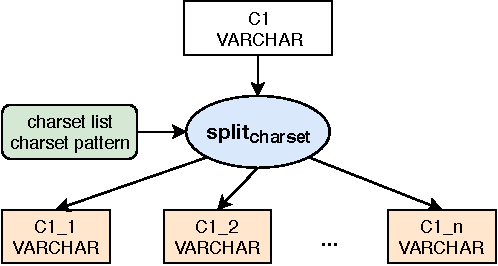
\includegraphics[width=1\linewidth]{expression_node-css-compression_2.pdf}
    \caption[b]{compression}
    \label{fig:pd:charsetsplit:exprnode:compression}
  \end{subfigure}
%   \hspace{1em}
  \begin{subfigure}[t]{0.49\linewidth}
    \centering
    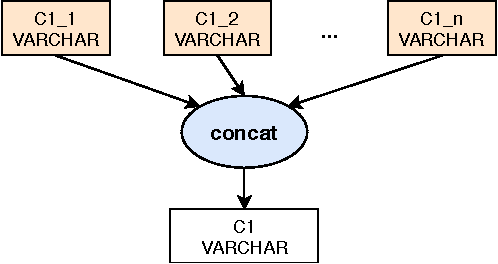
\includegraphics[width=1\linewidth]{expression_node-css-decompression_2.pdf}
    \caption[b]{decompression}
    \label{fig:pd:charsetsplit:exprnode:decompression}
  \end{subfigure}
  \caption{Character set split expression nodes}
  \label{fig:pd:charsetsplit:exprnode}
\end{figure}

The \textit{compression node} takes as input the string column and the compression metadata and outputs \(n\) \verb|VARCHAR| columns, where \(n = \mathit{len}(charset_{pattern})\)---one column for each character group. The \textit{decompression node} takes as input the \(n\) columns and concatenates them to reconstruct the original input column.

The compression operator \(split_{charset}\) takes as input the string value \(v_{s}\) and the compression metadata: \(charset_{list}\) and \(charset_{pattern}\). It applies the \textit{get\_charset\_pattern} function on \(v_{s}\) to obtain \(charset_{pattern}\_v\). It then compares \(charset_{pattern}\_v\) with \(charset_{pattern}\) to see if \(v_{s}\) has the correct structure. If they are not equal, it raises an \textit{OperatorException}, indicating that \(v_{s}\) is an exception. Otherwise, it splits \(v_{s}\) into \(n\) substrings---each one corresponding to a charset group---and returns them. The decompression operator \(concat\) receives as input \(n\) substrings and concatenates them to reconstruct the original value \(v_{s}\).

This representation scheme does not bring any compression benefit by itself. Instead, it creates compression opportunities by splitting columns into sub-columns that can be recursively compressed with other techniques. E.g. the columns in Table~\ref{tab:pd:charsetsplit:examples} can be compressed as follows:\\
1) the \textit{customer} column is first split into 2 columns: \textit{letters} and \textit{digits}. Then the \textit{letter} column is represented as a \nameref{subsec:pd:constant} and the \textit{digits} column is represented through a \nameref{subsec:pd:numericstrings} node and further compressed with numeric compression schemes (e.g. DELTA).\\
2) the \textit{account} column is split into 3 columns: \textit{letters}, \textit{digits}, \textit{spaces}. The \textit{letters} column gets compressed with \nameref{subsec:pd:dict} encoding. The \textit{digits} column is compressed similarly to the one in the \textit{customer} column. The \textit{spaces} column may be compressed through a custom representation scheme that identifies values with a single repeated character and only stores their number, or, alternatively, through \nameref{subsec:pd:dict} encoding, since the number of different space padding sequences is most likely small.\\
3) the \textit{transaction} column is split into 4 \textit{delimiter} columns and 3 \textit{hex} columns. All \textit{delimiter} columns have only 1 constant character and are compressed as \nameref{subsec:pd:constant}. The \textit{hex} columns can be represented through an implementation of \nameref{subsec:pd:numericstrings} that supports hexadecimal numbers, leading to 3 numeric columns that can benefit from numeric compression schemes.\\
In all three cases the \nameref{subsec:pd:charsetsplit} representation transforms an uncompressible \verb|VARCHAR| column into multiple compressed physical columns, significantly reducing the disk space required to store the data.

% ---------------------------------------------------------------------------
% ----------------------- end of thesis sub-document ------------------------
% ---------------------------------------------------------------------------